\documentclass[letterpaper]{article}

    \usepackage{longtable}
    \usepackage{graphicx}
    \usepackage{multirow}
    \usepackage{framed}
    \usepackage{mdframed}
        \newmdenv[linecolor=blue,frametitle=Illustration, backgroundcolor=blue!03]{sample}
        \newmdenv[linecolor=black,frametitle=Commands, backgroundcolor=yellow!08]{cmd}
    \usepackage{xcolor}
    \usepackage{listings}
    \usepackage{amsmath}
    \usepackage{amsfonts}
    \usepackage{mathtools}
    \usepackage{textcomp}
    \usepackage{lipsum}
    \usepackage[top=1in, bottom=1.5in, left=1.75in, right=1.75in]{geometry}
    \usepackage{hyperref}
    \usepackage{endnotes}

    \usepackage{imakeidx}
    \makeindex{}

    \newtheorem{theorem}{Theorem}
    \newtheorem{proof}{Proof}
    \newtheorem{definition}{Definition}

    %this is a trick to print "\end{verbatim}" in a verbatim environment
    \usepackage{verbatim}
    \newenvironment{realverbatim}{\verbatim}{\endverbatim}

    %new commands
    \newcommand{\bib}{Bib\TeX}
    \newcommand{\Lx}{\LaTeXe}

    \title{Another Short Tutorial for \LaTeXe}
    \author{Charles Carter}
    \date{\today{}}

\begin{document}

    \maketitle{}
    
    \tableofcontents{}
    \listoffigures{}
    \listoftables{}

    \newpage{}

    \section{Introduction}
    \label{Introduction}

    Let's begin thinking about \Lx{}  by considering the concept of \textit{easy}. We don't often think of easiness as having a context, but it certainly does. For example, which is easier to use, a shovel and wheelbarrow, or an excavator and dump truck? If we were digging a hole to plant a bush we would choose the former, but if we were digging a swimming pool we would choose the latter. Again, which is easier to use, a pickup truck or an eighteen wheeler? If we were hauling a few garden supplies we would choose the former, but if we were hauling electric generators to California, we would choose the latter. Which is easier to use, a word processing program (e.g., Microsoft Word), or a professional typesetting program (e.g., \Lx{})? If we were writing a letter or a grocery list, we would choose the former, but if we were writing a mathematical, scientific, or engineering document, we would choose the latter. I can't say whether one choice is ``easier'' than the other, but I can say that it's easier to use the right tool for the job than to attempt a task using the wrong tool. It's in this spirit that I offer this tutorial. 

    This is a short, easy, nontechnical introduction to \LaTeXe{}. It's a tutorial designed for students who do not have a lot of time, who do not need to become overnight experts in \LaTeXe{}, and prefer a shallow learning curve to a boot camp approach.  After you have worked through it, you will be able to create professional documents, and have the ability to teach yourself how to extend your \LaTeXe{} skills --- to become a \LaTeXe{} guru if you want to or need to.

        \textbf{What about \Lx{}?} First, it's \textit{free} in the senses both that you do not have to pay for it and that you have the ability to change it without the permission of anyone. Second, it's \textit{easy}, given that you know how to use it. As always, there are trade-offs, and ``easy'' to an expert tends to be hard for a beginner, and \textit{vice versa}. Third, it's \textit{stable}, the first version released in 1985, and documents written four decades ago still compile today. Fourth, it's \textit{well documented}, not surprising since its purpose is document preparation. Fifth, it's \textit{professioal}, as you will soon come to see. Finally, \Lx{} is \textit{universal}. I will touch on these points from time to time in this tutorial.

    \textbf{How does this introduction work?} Each ``lesson'' consists of the introduction of a few commands, some text to copy, paste, and compile, and a couple of questions. Ech lesson should not take more than fifteen minutes to complete. It uses the ``baby talk'' principle --- you imitate what you see and explore it by making slight changes. If you complete one lesson a day, within several weeks you will have a good foundation with \LaTeXe{}, and begin to create professional quality documents. You will also see how the things I wrote in the preceding paragraph are true.

    Please note that this tutorial \textit{is not} a \LaTeXe{} reference; you will need to find a good reference that details the options and arguments for each command. It's also not a user guide. Nor is it a full introduction to \LaTeXe{}, although it will introduce it to students not previously familiar with it. It gives an ideosyncratic view of \LaTeXe{} (my own). It promises only to be short, easy, and useful, not long-winded or difficult, even if it does omit some very important details. 

        \section{Document Basics}
    \label{Document-Basics}

    A \texttt{tex} document consists of plain text, and special characters, commands, and environments. I will generally refer to special characters, commands, and enviormments with the word \textit{commands}; you don't need to know the difference between them now, but you shortly will without being told. You \textit{must} precede commands with a backslash (\textbackslash{}) for the compiler to know that they are commands. This is easy to forget, so I will remind you the first couple of times.

	\paragraph{What should I have?}You should have a working \LaTeXe{} program. If you do not have one, see Appendix \ref{Installing} below. You will also need a text editor, and you will probably want to get an integrated editor, compiler, and printer. See Appendix \ref{Development Environments}. You can also use the old fashioned command line, I cover this in Appendix \ref{Command Line}.

        \subsection{Basic document}
        \label{Basic-document}
        
        \begin{framed}
            \begin{itemize}
                \item{documentclass}
                \item{begin/end document}
				\item{plain text}
				\item{comments}
            \end{itemize}
        \end{framed}

        A basic document begins with a document class, and has a preamble and contents. Type (or copy) the following, save it as a \texttt{.tex} document and compile it. The percent signs (\%) are comments and do not have any effect on  the document.

        \begin{verbatim}
\documentclass{article}
    %this is the preamble
\begin{document}
    %this is the contents section
    It works! %plain text prints as it
\end{document}    
        \end{verbatim}

        \paragraph{Exercise:}\LaTeXe{} has a number of different document classes. Name four of them.

        \paragraph{Exercise:}A \texttt{documentclass} command can take optional arguments, like this: \texttt{documentclass[optional arguments]\{document class\}}.\footnote{Don't forget to type a backslash before the command, like this: \texttt{\textbackslash{}documentclass}} Name two optional arguments.

        \subsection{Basic title}
        \label{Basic-title}
        
        \begin{framed}
            \begin{itemize}
                \item{title}
                \item{author}
                \item{date}
                \item{maketitle}
            \end{itemize}
        \end{framed}

        A basic document usually title and author information in the preamble. You specify the title with the \texttt{title} command. You specify the author(s) with the \texttt{author} command. You may optionally specify a date with the \texttt{date} command. In the body of the document, you create the title with the \texttt{maketitle} command. Create and compile a second document like this:        

        \begin{verbatim}
\documentclass{article}
    \title{Title, Author, and Date}
    \author{Charles Carter}
    \date{July 4, 1776}
\begin{document} 
    \maketitle{}
    This document has a title, author, and date.
\end{document}    
        \end{verbatim}

        \paragraph{Exercise:}What happens if you use the command \texttt{today\{\}}\footnote{Remember, \texttt{\textbackslash{}date\{\}}} as the date parameter (replacing July 4, 1776)?

        \paragraph{Exercise:}What happens if you use the command \texttt{thanks\{email address\}}\footnote{\texttt{\textbackslash{}thanks\{\}}} after your name in the \texttt{author\{\}} command?

        \subsection{Basic sections}
        \label{Basic-sections}
        
        \begin{framed}
            \begin{itemize}
                \item{section}
                \item{subsection}
                \item{subsubsection}
                \item{label}
            \end{itemize}
        \end{framed}

        \LaTeXe{} provides a number of useful section levels, including part and chapter. Two of the most useful are \texttt{section} and \texttt{subsection}. Create and compile the following document. 

        The \texttt{label\{\}} is used to create cross-references in documents. It's also very helpful in organizing your thoughts. The argument to \texttt{label\{argument\}} does not appear in the document. I cover the \texttt{ref} and \texttt{pageref} commands below in subsection \ref{Footnotes} on page \pageref{Footnotes}. These are used to create references back to the label.

        \begin{verbatim}
\documentclass{article}
    \title{Basic Sections}
    \author{Charles Carter}
    \date{\today{}}
\begin{document} 
    \maketitle{}
    \section{Introduction}
    \label{Introduction}
    \section{Body}
    \label{Body}
    \section{Conclusion}
    \label{Conclusion}
\end{document}    
        \end{verbatim}

        \paragraph{Exercise:}What do the commands \texttt{subsection\{\}} and \texttt{subsubsection\{\}} do?

        \paragraph{Exercise:}What does \texttt{section*\{\}} do? Note the asterisk (*) after \texttt{section}. You can also use this starred version for \texttt{subsections} and \texttt{subsubsections}.

        \subsection{Basic paragraphs}
        \label{Basic-paragraphs}
        
        \begin{framed}
            \begin{itemize}
                \item{paragraph}
                \item{subparagraph}
            \end{itemize}
        \end{framed}


        We have reached the point where you need some real content. I will use the text of Abraham Lincoln's Gettysburg Address to illustrate paragraphs. Notice that ordinary paragraphs do not need a special commend -- the ``paragraph command'' is simply two blank lines to create an empty new line between the paragraphs, as if they were double spaced. Create and compile the following document.

        \begin{verbatim}
\documentclass{article}
    \title{Basic Paragraphs}
    \author{Charles Carter}
    \date{\today{}}
\begin{document} 
    \maketitle{}
    \section{Introduction}
    \label{Introduction}
    \section{Body}
    \label{Body}

Four score and seven years ago our fathers brought forth on this 
continent a new nation, conceived in liberty, and dedicated to 
the proposition that all men are created equal.

Now we are engaged in a great civil war, testing whether that nation, 
or any nation so conceived and so dedicated, can long endure. We 
are met on a great battlefield of that war. We have come to dedicate 
a portion of that field, as a final resting place for those who here 
gave their lives that that nation might live. It is altogether fitting 
and proper that we should do this.

But, in a larger sense, we can not dedicate, we can not consecrate, 
we can not hallow this ground. The brave men, living and dead, who 
struggled here, have consecrated it, far above our poor power to add 
or detract. The world will little note, nor long remember what we say 
here, but it can never forget what they did here. It is for us the 
living, rather, to be dedicated here to the unfinished work which they 
who fought here have thus far so nobly advanced. It is rather for us 
to be here dedicated to the great task remaining before us, that from 
these honored dead we take increased devotion to that cause for which 
they gave the last full measure of devotion, that we here highly resolve 
that these dead shall not have died in vain, that this nation, under 
God, shall have a new birth of freedom, and that government of the people, 
by the people, for the people, shall not perish from the earth.

    \section{Conclusion}
    \label{Conclusion}
\end{document}    
        \end{verbatim}
        
        \paragraph{Exercise:}What happens if you include the \texttt{paragraph\{\}} or \texttt{subparagraph\{\}} commands before each paragraph? 
        
        \paragraph{Exercise:}What happens if you include arguments with the \texttt{paragraph\{argument\}} or \texttt{subparagraph\{argument\}} commands? 

        \subsection{Basic packages}
        \label{Basic packages}
        
        \begin{framed}
            \begin{itemize}
                \item{usepackage}
                \item{lipsum}
            \end{itemize}
        \end{framed}

Much of \LaTeXe{} functionality is contained in external packages. To use this functionality, you include the command \texttt{usepackage\{\}} in the preamble. Of course, you first have to install the package on your computer, but the MiKTeX distribution does that automatically. The \texttt{lipsum} package generates generic text (in Latin, of course). The \texttt{lipsum\{\}} command generates text. Notice that you can control the number of paragraphs to include. Below, I have included paragraph $1$ in the introduction, paragraphs $2$ through $4$ in the body, and paragraph $5$ in the conclusion.

Notice the paragraph indentation. First paragraphs are \textit{not} indented. Following paragraphs \textit{are} indented. This is normal typographic practice.

        \begin{verbatim}
\documentclass{article}
    \usepackage{lipsum}
    \title{Using Packages}
    \author{Charles Carter}
    \date{\today{}}
\begin{document} 
    \maketitle{}
    \section{Introduction}
    \label{Introduction}
        \lipsum[1]{}
    \section{Body}
    \label{Body}
        \lipsum[2-4]{}
    \section{Conclusion}
    \label{Conclusion}
        \lipsum[5]{}
\end{document}    
        \end{verbatim}

        \paragraph{Exercise:}What is CTAN, the Comprehensive \TeX{} Archive Network? How many packages are currently on CTAN?

        \paragraph{Exercise:}What are the most popular \LaTeXe{} packages?

        \subsection{Basic contents}
        \label{Basic contents}
        
        \begin{framed}
            \begin{itemize}
                \item{tableofcontents}
            \end{itemize}
        \end{framed}

        Creating a table of contents is easy. Just include the \texttt{tableofcontents\{\}} command. You may have to compile the document twice to ensure that the table of contents is generated properly.
        \begin{verbatim}
\documentclass{article}
    \usepackage{lipsum}
    \title{Table of Contents}
    \author{Charles Carter}
    \date{\today{}}
\begin{document} 
    \maketitle{}
    \tableofcontents{}
    \section{Introduction}
    \label{Introduction}
        \lipsum[1]{}
    \section{Body}
    \label{Body}
        \lipsum[2-4]{}
    \section{Conclusion}
    \label{Conclusion}
        \lipsum[5]{}
\end{document}    
        \end{verbatim}

        \paragraph{Exercise:}The \texttt{section[argument]\{Section Title\}} command takes an optional argument. How does this argument affect the table of contents?

        \paragraph{Exercise:}What other kinds of content tables can \LaTeXe{} generate? To start with, look at figures and tables.

        \subsection{Basic decorations}
        \label{Basic decorations}
        
        \begin{framed}
            \begin{itemize}
                \item{textit}
                \item{textsf}
                \item{texttt}
                \item{textbf}
                \item{textsc}
                \item{underline}
            \end{itemize}
        \end{framed}

In this section, you will fiddle with the appearance of text. To \textit{create text in italics}, use \texttt{textit}. To \textsf{create text in sans serif}, use \texttt{textsf}. To \texttt{create text in monospace font}, use \texttt{texttt}. To \textbf{create text in boldface}, use \texttt{textbf}. To \textsc{create text using Small Caps}, use \texttt{textsc}. \underline{You should almost never underline text}! If you choose to do so, use \texttt{underline}.

        \paragraph{}To \textit{create text in italics}, use \texttt{textit}. 
        \paragraph{}To \textsf{create text in sans serif}, use \texttt{textsf}. 
        \paragraph{}To \texttt{create text in monospace font}, use \texttt{texttt}. 
        \paragraph{}To \textbf{create text in boldface}, use \texttt{textbf}. 
        \paragraph{}To \textsc{create text using Small Caps}, use \texttt{textsc}. 
        \paragraph{}\underline{You should almost never underline text}! If you choose to do so, use \texttt{underline}.

        \begin{verbatim}
\documentclass{article}
    \title{Font Appearance}
    \author{Charles Carter}
    \date{\today{}}
\begin{document} 
    \maketitle{}
    \section{Introduction}
    \label{Introduction}
    \section{Body}
    \label{Body}
        \paragraph{}In this section, you will fiddle with the appearance of text. 
        \paragraph{}To \textit{create text in italics}, use \texttt{textit}. 
        \paragraph{}To \textsf{create text in sans serif}, use \texttt{textsf}. 
        \paragraph{}To \texttt{create text in monospace font}, use \texttt{texttt}. 
        \paragraph{}To \textbf{create text in boldface}, use \texttt{textbf}. 
        \paragraph{}To \textsc{create text using Small Caps}, use \texttt{textsc}. 
        \paragraph{}\underline{You should almost never underline text}! 
        If you choose to do so, use \texttt{underline}.
    \section{Conclusion}
    \label{Conclusion}
\end{document}    
        \end{verbatim}

        \paragraph{Exercise:}As with much else in \LaTeXe,there are multiple ways to italisize or bold-face text. Can you find other ways?



        \subsection{Basic fontsizes}
        \label{Basic fontsizes}
        
        \begin{framed}
            \begin{itemize}
                \item{tiny}
                \item{scriptsize}
                \item{footnotesize}
                \item{small}
                \item{normalsize}
                \item{large}
                \item{Large}
                \item{LARGE}
                \item{huge}
                \item{Huge}
            \end{itemize}
        \end{framed}

\LaTeXe{} has several different ways to alter the size of the font. Perhaps the simplest way is to create a \textit{size environment}. You do this by using one of the commands listed above, and this controls the size of all text until it is changed by another command. You would typically use this for sections of text that need to be made smaller, such as tables, block quotes, technical sections not germane to the main discussion, and similar.

    \normalsize{}\paragraph{}This paragraph has a normalsize font size.
    \tiny{}\paragraph{}This paragraph has a tiny font size.
    \scriptsize{}\paragraph{}This paragraph has a scriptsize font size.
    \footnotesize{}\paragraph{}This paragraph has a footnotesize font size.
    \small{}\paragraph{}This paragraph has a small font size.
    \normalsize{}\paragraph{}This paragraph has a normalsize font size.
    \large{}\paragraph{}This paragraph has a large font size.
    \Large{}\paragraph{}This paragraph has a Large font size.
    \LARGE{}\paragraph{}This paragraph has a LARGE font size.
    \huge{}\paragraph{}This paragraph has a huge font size.
    \Huge{}\paragraph{}This paragraph has a Huge font size.
    \normalsize{}\paragraph{}This paragraph has a normalsize font size.

        \begin{verbatim}
\documentclass{article}
    \title{Font Sizes}
    \author{Charles Carter}
    \date{\today{}}
\begin{document} 
    \maketitle{}
    \section{Introduction}
    \label{Introduction}
    \section{Body}
    \label{Body}
    \normalsize{}\paragraph{}This paragraph has a normalsize font size.
    \tiny{}\paragraph{}This paragraph has a tiny font size.
    \scriptsize{}\paragraph{}This paragraph has a scriptsize font size.
    \footnotesize{}\paragraph{}This paragraph has a footnotesize font size.
    \small{}\paragraph{}This paragraph has a small font size.
    \normalsize{}\paragraph{}This paragraph has a normalsize font size.
    \large{}\paragraph{}This paragraph has a large font size.
    \Large{}\paragraph{}This paragraph has a Large font size.
    \LARGE{}\paragraph{}This paragraph has a LARGE font size.
    \huge{}\paragraph{}This paragraph has a huge font size.
    \Huge{}\paragraph{}This paragraph has a Huge font size.
    \normalsize{}\paragraph{}This paragraph has a normalsize font size.
    \section{Conclusion}
    \label{Conclusion}
\end{document}    
        \end{verbatim}

        \paragraph{Exercise:} The issues of font, font size, and font decoration, are difficult, complicated, and subject to internecene wars. You may want to postpone your exploration of these issues until you have created and compiled several hundred \texttt{.tex} documents. If you want, and have discretionary time available and nothing else to do, you may want to delve into the complex and divisive world of fonts, font sizes, and font decorations.



    \section*{\LaTeXe{} is \textit{Universal}}

        \section{Math and Symbols}
    \label{Math}

	Both \TeX{} and \Lx{} shine when it comes to math. In fact, Donald Knuth originally wrote \TeX{} just so he could typeset math. In this section, we will dip our toes into math and symbols. This will not be difficult. If you have need for more advanced mathematics, you will know how to find what you need to render your equations.

        \subsection{Special characters}
        \label{Special-characters}
        
		Most characters are not special. An \textit{a} is just an a, a \textit{Z} is just a Z, and a \textit{7} is just a 7. Sometimes, this isn't the case --- an \&  is not just an ampersand. \Lx{} has ten special characters. They are listed below.

        \begin{cmd}
            \begin{itemize}
                \item backslash - \textbackslash
                \item  percent - \%
                \item  left curly bracket - \{
                \item  right curly bracket - \}
                \item  dollar sign - \$
                \item  caret - \^{} 
                \item  underscore - \_
                \item  tilde - \~{} 
                \item  hash - \#
                \item  ampersand - \&
                \index{\textbackslash}
                \index{\%}
                \index{\{\}}
                \index{\$}
                \index{\^{}}
                \index{\_}
                \index{\#}
                \index{\&}
            \end{itemize}
        \end{cmd}

        You already lnow four of them. ``\textbackslash'' indicates the beginning of a command, ``\%'' indicates a comment, and the ``\{ \ldots{} \}'' pair (usually) indicates the argument to a command. You will learn about three more in this section, the dollar sign ``\$'', the underscore ``\_'', and the caret ``\^{}''. It's worthwhile to stare at these ten characters long enough to become familiar with them. When your document misbehaves, often these characters are the culprit.

		Sometimes you will find characters that wish they were special, but are not. These include the cedilla (\c{c}), the degree (\textdegree), and diphthongs (\ae). All these are represented by \Lx{} commands, you will use the command for the character.

		\paragraph{Exercise:}Scott Pakin has published the booklet \textit{The Comprehensiv \LaTeX{} Symbol List}. You can find this online in PDF format. Search for it and just look at it. It contains over 300 pages of symbols. You'll be amazed! 

        \subsection{Inline math}
        \label{Inline-math}
        
        \begin{cmd}
            \begin{itemize}
                \index{\$}
                \index{+}
                \index{plus}
				\index{- (dash or subtraction)}
                \index{times}
                \index{ast}
                \index{cdot}
                \index{frac or div}
                \index{sqrt}
				\index{\^{} (caret or circumflex)}
				\index{\_ (underscore)} 
                \item{\$}
                \item{plus or +}
				\item{- (dash or subtraction)}
                \item{times or ast or cdot}
                \item{frac or div}
                \item{sqrt}
				\item{\^{} (caret or circumflex)}
				\item{\_ (underscore)} 
            \end{itemize}
        \end{cmd}

        These commands represent the basic arithmetic operations of addition, subtraction, multiplication, and division. These also include the square root and exponents.
        \begin{sample}
	This is an example of inline math.\\
Use the dollar symbol (\$) to set the math.\\
Here is how it works.\\
 Addition: $4 + 5 = 9$.\\
 Subtraction: $4 - 5 = -1$.\\
 Multiplication: $4 \times 5 = 20$.\\
Multiplication: $4 \cdot 5 = 20$.\\
 Multiplication: $4 \ast 5 = 20$.\\
 Division: $\frac{4}{5} = 0.8$.\\
 Division: $4 \div 5 = 0.8$.\\
 Square root: $\sqrt{2} = 1.41421$.\\
 Higher roots: $\sqrt[4]{81} = 3$.\\
 Exponents: $2^8 = 256$.\\
 Subscripts: $x_0, x_1, x_2$.
        \end{sample}

        \begin{verbatim}
\documentclass{article}
    \title{Inline Math}
    \author{Charles Carter}
    \date{\today{}}
\begin{document} 
    \maketitle{}
	This is an example of inline math. Use the dollar symbol (\$) to set the math. \\
	Here is how it works. \\
    Addition: $4 + 5 = 9$. \\
    Subtraction: $4 - 5 = -1$. \\
    Multiplication: $4 \times 5 = 20$. \\
    Multiplication: $4 \cdot 5 = 20$. \\
    Multiplication: $4 \ast 5 = 20$.\\
    Division: $\frac{4}{5} = 0.8$. \\
    Division: $4 \div 5 = 0.8$. \\
    Square root: $\sqrt{2} = 1.41421$. \\
    Higher roots: $\sqrt[4]{81} = 3$.\\
    Exponents: $2^8 = 256$.\\
	Subscripts: $x_0, x_1, x_2$
\end{document}    
		\end{verbatim}

		\paragraph{Exercise:} You can find the \textit{User's Guide for the }\texttt{amsmath} \textit{Package} in PDF format online. Search for it and start reading through it.

        \subsection{Equations}
        \label{Equations}
        
        \begin{cmd}
            \begin{itemize}
                \index{amsmath}
                \index{equation}
                \index{equation*}
                \item{amsmath}
                \item{equation}
                \item{equation*}
            \end{itemize}
        \end{cmd}
	
		\Lx{} provides the \textit{equation} environment for writing block equations with the \textit{amsmath} package. First, import the package with \texttt{usepackage\{amsmath\}}.  Equations are numbered and can be referenced by means of their labels. The starred version omits the equation from the numbered equations. Here are some examples. Equation \ref{line} is the formula for a straight line. Equation \ref{slope} is the formula for the slope of a straight line.  The third, unnumbered equation is the formula for a straight line with multiple parameters.

        \begin{sample}
		\begin{equation}
			\label{line}
			y = \beta_0 + \beta_1 x_1
		\end{equation}
		\begin{equation}
			\label{slope}
			m = \frac{y_1 - y_0}{x_1 - x_0}
		\end{equation}
		\begin{equation*}
			y = \beta_0 + \beta_1 x_1 + \beta_2 x_2 + \beta_3 x_3
		\end{equation*}
        \end{sample}

        \begin{verbatim}
\documentclass{article}
	\usepackage{amsmath}
    \title{Equations}
    \author{Charles Carter}
    \date{\today{}}
\begin{document} 
    \maketitle{}
	This is an example of equations.
		\begin{equation}
			\label{line}
			y = \beta_0 + \beta_1 x_1
		\end{equation}
		\begin{equation}
			\label{slope}
			m = \frac{y_1 - y_0}{x_1 - x_0}
		\end{equation}
		\begin{equation*}
			y = \beta_0 + \beta_1 x_1 + \beta_2 x_2 + \beta_3 x_3
		\end{equation*}
	\end{document}    
        \end{verbatim}

		\paragraph{Exercise:}Continue reading through the \textit{User's Guide for the }\texttt{amsmath} \textit{Package}.

        \subsection{Multiline equations}
        \label{Multiline equations}
        
        \begin{cmd}
            \begin{itemize}
                \index{align}
                \index{gather}
                \index{multline}
                \item{align}
                \item{gather}
                \item{multline}
            \end{itemize}
        \end{cmd}

		How do I place several equations together in one equation environment, aligned on a particular character, such as an equal sign (=)? Use the \textit{align} environment, with the ampersand (\&) as the tab character, and end each line with two backslashs (\textbackslash{}\textbackslash{}).

        \begin{sample}
		\begin{align}
			y& = \beta_0 + \beta_1 x_1\\
			slope& = \frac{y_1 - y_0}{x_1 - x_0}\\
			predictedvalue& = \beta_0 + \beta_1 x_1 + \beta_2 x_2 + \beta_3 x_3
		\end{align}
        \end{sample}

		How to I center the equations? Use the \textit{gather} environment, with no tab character but ending each line with two backslashes (\textbackslash{}\textbackslash{}).

        \begin{sample}
		\begin{gather}
			y = \beta_0 + \beta_1 x_1\\
			slope = \frac{y_1 - y_0}{x_1 - x_0}\\
			predictedvalue = \beta_0 + \beta_1 x_1 + \beta_2 x_2 + \beta_3 x_3
		\end{gather}
        \end{sample}

		What if I have a very long equation that won't fit on one line? Use the \textit{multiine} environment, breaking with two backslashes (\textbackslash{}\textbackslash{})

        \begin{sample}
		\begin{multline}
			y = \beta_0 + \beta_1 x_1 + \beta_2 x_2 + \beta_3 x_3 +\\
			\beta_4 x_4 + \beta_5 x_5 + \beta_6 x_6 +\\
			\beta_7 x_7 + \beta_8 x_8 + \beta_9 x_9
		\end{multline}
        \end{sample}
		
		\begin{verbatim}
\documentclass{article}
	\usepackage{amsmath}
    \title{Multiline Equations}
    \author{Charles Carter}
    \date{\today{}}
\begin{document} 
    \maketitle{}
	This is an example of align.
		\begin{align}
			y& = \beta_0 + \beta_1 x_1\\
			slope& = \frac{y_1 - y_0}{x_1 - x_0}\\
			predictedvalue& = \beta_0 + \beta_1 x_1 + \beta_2 x_2 + \beta_3 x_3
		\end{align}
	This is an example of gather.
		\begin{gather}
			y = \beta_0 + \beta_1 x_1\\
			slope = \frac{y_1 - y_0}{x_1 - x_0}\\
			predictedvalue = \beta_0 + \beta_1 x_1 + \beta_2 x_2 + \beta_3 x_3
		\end{gather}
	This is an example of multline.
		\begin{multline}
			y = \beta_0 + \beta_1 x_1 + \beta_2 x_2 + \beta_3 x_3 +\\
			\beta_4 x_4 + \beta_5 x_5 + \beta_6 x_6 +\\
			\beta_7 x_7 + \beta_8 x_8 + \beta_9 x_9
		\end{multline}
	\end{document}    
        \end{verbatim}

        \subsection{Higher math}
        \label{Higher math}
        
        \begin{cmd}
            \begin{itemize}
                \index{sums}
                \index{products}
                \index{limits}
                \index{derivatives}
                \index{integrals}
                \item{sums}
                \item{products}
                \item{limits}
                \item{derivatives}
                \item{integrals}
            \end{itemize}
        \end{cmd}

		Equation \ref{higher:sum} states the shorthand for the sum of a series of integers 1 through $n$. Equation \ref{higher:prod} states the shorthand for the product of a series of integeers 1 through $n$. Equation \ref{higher:lim} demonstrates the notation for limits. Equation \ref{higher:deriv} demonstrates the notation for derivatives. Equation \ref{higher:int} demonstrates the notation for integrals.

        \begin{sample}
		\begin{gather}
			\sum_{i=1}^{i=n} i = 1 + 2 + 3 + \dotsm{} + n \label{higher:sum} \\
			\prod_{i=1}^{i=n} i = 1 \times 2 \times 3 \times \dotsm{} \times n \label{higher:prod} \\
			\lim_{x \to \infty} f(x) \label{higher:lim} \\
			\frac{d}{dx} \left[ e^\frac{x}{2} sin(ax)\right] \label{higher:deriv} \\
			\int_{a}^{b} x^2 dx \label{higher:int}
		\end{gather}
        \end{sample}
		

        \begin{verbatim}
\documentclass{article}
    \usepackage{amsmath}
    \title{Higher Math}
    \author{Charles Carter}
    \date{\today{}}
\begin{document} 
    \maketitle{}
		\begin{gather}
			\sum_{i=1}^{i=n} i = 1 + 2 + 3 + \dotsm{} + n \\
			\prod_{i=1}^{i=n} i = 1 \times 2 \times 3 \times \dotsm{} \times n \\
			\lim_{x \to \infty} f(x) \label{higher:lim} \\
			\frac{d}{dx} \left[ e^\frac{x}{2} sin(ax)\right] \\
			\int_{a}^{b} x^2 dx
		\end{gather}
\end{document}    
        \end{verbatim}

		\paragraph{Exercise:}Continue reading through the \textit{User's Guide for the }\texttt{amsmath} \textit{Package}.

        \subsection{Theorems, etc.}
        \label{Theorems}
        
        \begin{cmd}
            \begin{itemize}
                \index{amsthm package}
                \index{package amsthm}
                \index{newtheorem}
                \index{addcontentsline}
                \item{amsthm package}
                \item{newtheorem}
                \item{addcontentsline}
            \end{itemize}
        \end{cmd}

        Stating theorems, lemmas, proofs, axioms, and similar constructions in \Lx{} is particularly easy. For simple applications, just define whatever environment you need in the preamble with \texttt{newtheorem}, like this: \texttt{newtheorem\{first argument\}\{second argument\}}. The \textit{first argument} is the name of the structure: theorem, lemma, definition, etc. The \textit{second argument} is the printed heading that the reader will see in the document.

        For more flexibility (and I do mean a \textit{lot} more flexibility) use the \texttt{amsthm} package, imported as usual in the preamble with \texttt{usepackage\{amsthm\}}. This package allows many customizations, for example, numbering by section and subsection, and concurrent numbering of theorems and proofs. The documentation of this package is fairly short and not overly complex, so it's not hard to read, understand, and use.

        Finally, you might want to add your theorem to the table of contents, Use \texttt{addcontentsline\{first argument\}\{second argument\}\{third argument\}}. The \textit{first argument} is the listing where you want the entry to appear: table of contents, list of tables, or list of figures. The \textit{second argument} is the kind of entry you want, such as section, subsection, etc. The \textit{third argument} is the printed text that will appear in the contents section.

        \begin{sample}
    \begin{theorem}
        \label{thm:first}
        \addcontentsline{toc}{subsubsection}{Fundamental Theorem of Calculus}
        Definite integral of a function is related to its antiderivative, and can be reversed by differentiation.
    \end{theorem}
    \begin{proof}
        \label{prf:first}
        \addcontentsline{toc}{subsubsection}{Proof of Fundamental Theorem of Calculus}
        If $f$ is continuous on $[a, b]$, 
            then $\int_a^b f$ exists. \\
        If $f$ is continous on $[a, b]$ and $c \in [a, b]$, 
            then $\int_a^c F + \int_c^b F = \int_a^b F$. \\
        If $m \leq f \leq M$ on $[a, b]$, 
            then $(b - a)m \leq \int_a^b f \leq (b - a)M$.
    \end{proof}
    \begin{definition}
        \label{def:first}
        \addcontentsline{toc}{subsubsection}{Definition of Calculus}
        Calculus is the branch of mathematics that deals with the finding and properties of derivatives and integrals of functions, by methods originally based on the summation of infinitesimal differences. The two main types are differential calculus and integral calculus.
    \end{definition}
    For the definition of calculus, see definition \ref{def:first}. For the fundamental theorem of calculus, see theorem \ref{thm:first}. For the proof, see proof \ref{prf:first}.
        \end{sample}
		

        \begin{verbatim}
\documentclass{article}
    \usepackage{amsmath}
    \newtheorem{theorem}{Theorem}
    \newtheorem{proof}{Proof}
    \newtheorem{definition}{Definition}
    \title{Theorems, Proofs, Definitions, etc.}
    \author{Charles Carter}
    \date{\today{}}
\begin{document}
    \maketitle{}
    Theorems, proofs, definitions, etc.  can easily be defined
    \begin{theorem}
        \label{thm:first}
        \addcontentsline{toc}{subsubsection}{Fundamental Theorem of Calculus}
        Definite integral of a function is related to its antiderivative, 
        and can be reversed by differentiation.
    \end{theorem}
    \begin{proof}
        \label{prf:first}
        \addcontentsline{toc}{subsubsection}{Proof of Fundamental Theorem of Calculus}
        If $f$ is continuous on $[a, b]$, 
            then $\int_a^b f$ exists. \\
        If $f$ is continous on $[a, b]$ and $c \in [a, b]$, 
            then $\int_a^c F + \int_c^b F = \int_a^b F$. \\
        If $m \leq f \leq M$ on $[a, b]$, 
            then $(b - a)m \leq \int_a^b f \leq (b - a)M$.
    \end{proof}
    \begin{definition}
        \label{def:first}
        \addcontentsline{toc}{subsubsection}{Definition of Calculus}
        Calculus is the branch of mathematics that deals with the 
        finding and properties of derivatives and integrals of 
        functions, by methods originally based on the summation 
        of infinitesimal differences. The two main types are 
        differential calculus and integral calculus.
    \end{definition}
    For the definition of calculus, see definition \ref{def:first}. 
    For the fundamental theorem of calculus, see theorem \ref{thm:first}. 
    For the proof, see proof \ref{prf:first}.
    \end{document}
        \end{verbatim}

        \paragraph{Exercise:} Create your own new theorem class, called Problem, perhaps, and write a problem.

        \paragraph{Exercise:} Access the documentation to the amsthm package and look through it.


        \subsection{Matrices}
        \label{Matrices}
        
        \begin{cmd}
            \begin{itemize}
                \index{vmatrix}
                \index{pmatrix}
                \index{bmatrix}
                \index{Bmatrix}
                \index{Vmatrix}
                \item{vmatrix}
                \item{pmatrix}
                \item{bmatrix}
                \item{Bmatrix}
                \item{Vmatrix}
            \end{itemize}
        \end{cmd}

        Matrices are contained within a math environment, either an equation block or inline math pairs (\$\ldots\$). They are entered by row. Each row ends with two backslash symbols (\textbackslash\textbackslash). Each element on a row is separaated by an ampersand (\&). The different variations create different surrounding brackets.
        \texttt{vmatrix} uses vertical bars ($|\ldots|$), for example, to indicate the determinant of the matrix.
        \texttt{pmatrix} uses parentheses [(\ldots)].
        \texttt{bmatrix} uses square brackets ([\ldots]).
        \texttt{Bmatrix} uses curly braces (\{\ldots\}).
        \texttt{Vmatrix} uses double vertical bars ($||\ldots||$).
        
        \begin{sample}
        $ \begin{bmatrix}
            1 & 3 & 3 \\
            1 & 4 & 3 \\
            1 & 3 & 4 
        \end{bmatrix}
         \times 
         \begin{bmatrix}
             7 & -3 & -3 \\
             -1 & 1 & 0 \\
             -1 & 0 & 1
         \end{bmatrix}
         =
         \begin{bmatrix}
             1 & 0 & 0 \\
             0 & 1 & 0 \\
             0 & 0 & 1
         \end{bmatrix} $
        \end{sample}

        \begin{verbatim}
\documentclass{article}
    \usepackage{amsmath}
    \title{Matrices}
    \author{Charles Carter}
    \date{\today{}}
\begin{document} 
    \maketitle{}
        $ \begin{bmatrix}
            1 & 3 & 3 \\
            1 & 4 & 3 \\
            1 & 3 & 4 
        \end{bmatrix}
         \times 
         \begin{bmatrix}
             7 & -3 & -3 \\
             -1 & 1 & 0 \\
             -1 & 0 & 1
         \end{bmatrix}
         =
         \begin{bmatrix}
             1 & 0 & 0 \\
             0 & 1 & 0 \\
             0 & 0 & 1
         \end{vmatrix} $
\end{document}    
        \end{verbatim}

		\paragraph{Exercise:}Continue reading through the \textit{User's Guide for the }\texttt{amsmath} \textit{Package}.

        \subsection{Greek letters}
        \label{Greek letters}
        
        Here are the Greek letters commonly used in mathematical and scientific applications, table \ref{table:Greek letters} on page \pageref{table:Greek letters}. The \Lx{} commands for the Greek letters are in inline math mode, so you \textit{must} surround the command by a pair of dollar signs (\$\ldots\$). You must also use the \texttt{amsmath} package.

        \begin{table}[!ht]
            \label{table:Greek letters}
        \begin{tabular}{|| l || l | l || l | l ||}
            \hline
            Name & UC command & UC Letter      & LC command & LC letter \\
            \hline
            \hline
            Alpha & Alpha & $A$      & alpha & $\alpha$ \\
            \hline
            Beta & B & $B$     & beta & $\beta$ \\
            \hline
            Gamma & Gamma & $\Gamma$     & gamma & $\gamma$ \\
            \hline
            Delta & Delta & $\Delta$     & delta & $\delta$ \\
            \hline
            Epsilon & E & $E$     & epsilon & $\epsilon$ \\
            \hline
            Zeta & Z & $Z$     & zeta & $\zeta$ \\
            \hline
            Eta & H  & $H$     & eta & $\eta$ \\
            \hline
            Theta & Theta & $\Theta$    & theta & $\theta$ \\
            \hline
            Iota & I & $I$     & iota & $\iota$ \\
            \hline
            Kappa & K & $K$     &  kappa & $\kappa$ \\
            \hline
            Lamba & Lambda & $\Lambda$    & lambda & $\lambda$ \\
            \hline
            Mu  & M & $M$     & mu & $\mu$ \\
            \hline
            Nu & N & $N$     & nu & $\nu$ \\
            \hline
            Xi & Xi & $\Xi$     & xi & $\xi$ \\
            \hline
            Omicron & O & $O$    & o & $o$ \\
            \hline
            Pi & Pi & $\Pi$     & pi & $\pi$ \\
            \hline
            Rho & R & $R$    & rho & $\rho$ \\
            \hline
            Sigma & S & $S$    & sigma & $\sigma$ \\
            \hline
            Tau & T & $T$    & tau & $\tau$ \\
            \hline
            Upsilon & Y & $Y$    & upsilon & $\upsilon$ \\
            \hline
            Phi & Phi & $\Phi$     & phi & $\phi$ \\
            \hline
            Chi & X & $X$     & chi & $\chi$ \\
            \hline
            Psi & Psi & $\Psi$     & psi & $\psi$ \\
            \hline
            Omega & Omega & $\Omega$    & omega & $\omega$ \\
            \hline
        \end{tabular}
            \caption{Greek letters}
        \end{table}

        \begin{verbatim}
\documentclass{article}
    \usepackage{amsmath}
    \title{Greek Letters}
    \author{Charles Carter}
    \date{\today{}}
\begin{document} 
    \maketitle
        \begin{tabular}{|| l || l | l || l | l ||}
            \hline
            Name & UC command & UC Letter      & LC command & LC letter \\
            \hline
            \hline
            Alpha & Alpha & $A$      & alpha & $\alpha$ \\
            \hline
            Beta & B & $B$     & beta & $\beta$ \\
            \hline
            Gamma & Gamma & $\Gamma$     & gamma & $\gamma$ \\
            \hline
            Delta & Delta & $\Delta$     & delta & $\delta$ \\
            \hline
            Epsilon & E & $E$     & epsilon & $\epsilon$ \\
            \hline
            Zeta & Z & $Z$     & zeta & $\zeta$ \\
            \hline
            Eta & H  & $H$     & eta & $\eta$ \\
            \hline
            Theta & Theta & $\Theta$    & theta & $\theta$ \\
            \hline
            Iota & I & $I$     & iota & $k\iota$ \\
            \hline
            Kappa & K & $K$     &  kappa & $\kappa$ \\
            \hline
            Lamba & Lambda & $\Lambda$    & lambda & $\lambda$ \\
            \hline
            Mu  & M & $M$     & mu & $\mu$ \\
            \hline
            Nu & N & $N$     & nu & $\nu$ \\
            \hline
            Xi & Xi & $\Xi$     & xi & $\xi$ \\
            \hline
            Omicron & O & $O$    & o & $o$ \\
            \hline
            Pi & Pi & $\Pi$     & pi & $\pi$ \\
            \hline
            Rho & R & $R$    & rho & $\rho$ \\
            \hline
            Sigma & S & $S$    & sigma & $\sigma$ \\
            \hline
            Tau & T & $T$    & tau & $\tau$ \\
            \hline
            Upsilon & Y & $Y$    & upsilon & $\upsilon$ \\
            \hline
            Phi & Phi & $\Phi$     & phi & $\phi$ \\
            \hline
            Chi & X & $X$     & chi & $\chi$ \\
            \hline
            Psi & Psi & $\Psi$     & psi & $\psi$ \\
            \hline
            Omega & Omega & $\Omega$    & omega & $\omega$ \\
            \hline
        \end{tabular}
\end{document}    
        \end{verbatim}

        \paragraph{Exercise:} Mathematics uses a large number of non-Latin characters. For example, search for the Hebrew character Aleph ($\aleph$) and the symbol for infinity ($\infty$).



    \section*{\LaTeXe{} is \textit{Professional}}

    \LaTeXe{} is flexible to an extreme. You can customize every part of your document. However, its authors have spent much time and effort to ensure that it gives a professional appearance ``out of the box.'' This short tutorial does not cover customization. After you have created and compiled several dozen \texttt{.tex} files, you will begin to see the need for customization.\footnote{The first thing you may want to do is to change the page margins. An easy way to change page margins is to use the \texttt{geometry package}, covered in section \ref{Geometry} on page \pageref{Geometry}}. Unless you have special requirements, such as page margins, paragraph spacing, and page page numbers, and you are happy with the appearance of your document, you do not need to think about customization.

    %references.tex
    
    \section{References}
    \label{References}

    In scientific and research writing, one of the most critical aspects is references. Think about it: can you imagine a research paper without a single reference? These include footnotes, endnotes, marginal notes, and especially citations to sources. References have two components, a target and a source, or a label and a reference to that label. We have used labels before, but now we will expicitly consider them.

    \subsection{Footnotes}
    \label{Footnotes}

        \begin{framed}
            \begin{itemize}
                \item{footnote}
                \item{label}
                \item{ref}
                \item{pageref}
            \end{itemize}
        \end{framed}

    To insert a footnote, just use the command \text{footnote}.\footnote{\label{references:fn}Don't forget to put the \textbackslash{} before the \texttt{footnote} command.} If you label the footnote, you can refer to the footnote by number and page in the text of the doucumemt. Please be sure to read footnote \ref{references:fn} on page \pageref{references:fn}.

        \begin{verbatim}
\documentclass{article}
    \title{Footnotes and References}
    \author{Charles Carter}
    \date{\today{}}
\begin{document} 
    \maketitle{}
    To insert a footnote, just use the command \text{footnote}.\footnote{\label{references:fn}
    Don't forget to put the \textbackslash{} before the \texttt{footnote} command.} If you 
    label the footnote, you can refer to the footnote by number and page in the text of the
    doucumemt. Please be sure to read footnote \ref{references:fn} on page 
    \pageref{references:fn}.
\end{document}    
        \end{verbatim}

        \paragraph{Exercise:} Read the \LaTeXe{} documentation on footnotes.

    \subsection{Endnotes}
    \label{Endnotes}
        
        \begin{framed}
            \begin{itemize}
                \item{package endnotes}
                \item{endnote}
                \item{theendnotes}
                \item{addcontentsline}
            \end{itemize}
        \end{framed}

    Endnotes are a little more complicated than footnotes, but not much.\endnote{The difference between footnotes and endnotes is that footnotes go at the foot of the page where they appear, whilc endnotes appear at the end of the document.} Here is an endnote.\endnote{This is an endnote.} In order to actually print the endnotes, use the \texttt{theendnotes} command. In order to create an entry for the endnotes in the table of contents, you must use the \texttt{addcontentsline}.\endnote{\label{references:en}The addcontentsline takes three parameters, where the line should be written, usually \textit{toc}, the formatting to be used, usually \textit{section}, and the name to be given to the entry, perhaps \textit{Endnotes}.} Please see endnote \ref{references:en} on page \pageref{references:en} for the details.

        \begin{verbatim}
\documentclass{article}
    \usepackage{endnotes}
    \title{Endnotes}
    \author{Charles Carter}
    \date{\today{}}
\begin{document} 
    \maketitle{}
    \tableofcontents{}
    \section{Text}
    Endnotes are a little more complicated than footnotes, but not much.\endnote{The 
    difference between footnotes and endnotes is that footnotes go at the foot of 
    the page where they appear, whilc endnotes appear at the end of the document.} 
    Here is an endnote.\endnote{This is an endnote.} In order to actually print 
    the endnotes, use the \texttt{theendnotes} command. In order to create an 
    entry for the endnotes in the table of contents, you must use the \texttt{addcontentsline}.
    \endnote{\label{references:en}The addcontentsline takes three parameters, 
    where the line should be written, usually \textit{toc}, the formatting to be 
    used, usually \textit{section}, and the name to be given to the entry, perhaps 
    \textit{Endnotes}.} Please see endnote \ref{references:en} on page 
    \pageref{references:en} for the details.
    \theendnotes{}
    \addcontentsline{toc}{section}{Endnotes}
\end{document}    
        \end{verbatim}

        \paragraph{Exercise:} Find and read through the documentation of the Endnotes package.

    \subsection{Margin notes}
    \label{Margin notes}

        \begin{framed}
            \begin{itemize}
                \item{marginpar}
                \item{reversemarginpar}
                \item{normalmarginpar}
                \item{raggedright}
            \end{itemize}
        \end{framed}

        \marginpar{Important point!}

        Marginal notes are really useful to call attention to very important points.  They can also be useful in drafting documents to note future edits, insertions, or deletions. Use \texttt{marginpar} to create a marginal note. To delete marginal notes during the drafting process, just comment them out. The text remains as a reminder of the modifications in the document.

        {\raggedright\reversemarginpar{\marginpar{This is reversed text}}}

        To permanantly reverse the page sides. use \texttt{reversemarginpar}. To reverse the reverse page margins, use \texttt{normalmarginpar}. To change the paragraph alignment from the default justified text, use the command \texttt{raggedright} in a block.

        {\raggedright\normalmarginpar\marginpar{This is in the correct margim}}

        \begin{verbatim}
\documentclass{article}
    \title{Margin Notes}
    \author{Charles Carter}
    \date{\today{}}
\begin{document} 
    \maketitle{}
        \marginpar{Important point!}
        Marginal notes are really useful to call attention to very important 
        points.  They can also be useful in drafting documents to note 
        future edits, insertions, or deletions. Use \texttt{marginpar} 
        to create a marginal note. To delete marginal notes during the 
        drafting process, just comment them out. The text remains as a 
        reminder of the modifications in the document.
        {\raggedright\reversemarginpar{\marginpar{This is reversed text}}}
        To permanantly reverse the page sides. use \texttt{reversemarginpar}.
        To reverse the reverse page margins, use \texttt{normalmarginpar}.
        {\raggedright\normalmarginpar\marginpar{This is in the correct margim}}
\end{document}    
        \end{verbatim}

        \paragraph{Exercise:} If you really need to create sophisticated marginal notes, you will need both the \texttt{geometry} and \texttt{marginnote} packages. The former is very useful, and you may need to use it in every paper. The latter is useful for marginal notes when you need something more than the default \LaTeXe{} commands.

    \subsection{Bibliography}
    \label{Bibliography}

        \begin{framed}
            \begin{itemize}
                \item{creating an external \bib{} database}
            \end{itemize}
        \end{framed}

    Needless to say, every research paper requires a bibliography. \LaTeXe{} has multiple ways to include bibliographies. I have chosen to use a method called \bib{}. There are three reasons for this choice. First. it's simple enough to include in a simple tutorial. Second, it gives good results using its default settings. Third, it's complex enough to be configured for almost any application (given an author's time and patience).

    \bib{} uses an external file as a bibliographical database. This means that management of the sources is separate from writing and editing the original document. The data from the external database is meerged into the original document with a series of commands. We will cover the basics of the external database in this lesson. In the following lesson, we will see how to merge the two files.

    The external \bib{} database is merely a plain text file with entries in a prescribed format. It \textit{must} have the \texttt{.bib} extension for the filename. The following file includes four books and three online sources. The \bib format file contains specifications for a large number of types of sources, and you should become familiar with the various types of documents and the format for each.    

    Create a document with the following content. Name it \texttt{tut.bib} and place it in the same directory with your original source document, where you compile your PDF output. Each entry has a type identifier followed by a curly brace pair (\{\ldots{}\}), within which are contained various fields separated by commas. The first field is the identifier you will use to access the entry. The subsequent fields are ``key''=``value'' pairs, giving the title, author, date etc.
    
        \begin{verbatim}
\\tut.bib
@book{
    goossens04,
    author    =  {Frank Mittelbach and 
        Michel Goossens and 
        Johannes Braams and 
        David Carlisle and 
        Chris Rowley},
    title     = {The \LaTeX{} Companion (Tools and Techniques for Computer Typesetting)},
    year      = {2004},
    edition =2nd},
    publisher = {Addison-Wesley},
    address   = {Reading, MA}
    ISBN      = {978-0201362992}
}
@book{
    kottwitz11,
    author    = {Stefan Kottwitz },
    title     = {\LaTeX{} Beginner's Guide},
    year      = {2011},
    publisher = {Packt Publishing},
    address   = {Birmingham, UK},
    ISBN      = {978-1847199867}
}
@book{
    kottwitz15,
    author    = {Stefan Kottwitz },
    title     = {\LaTeX{} Cookbook},
    year      = {2015},
    publisher = {Packt Publishing},
    address   = {Birmingham, UK},
    ISBN      = { 978-1784395148}
}
@book{
    gratzer14,
    author    = {George Gr{\''a}tzer},
    title     = {Practical \LaTeX{}},
    year      = {2014},
    publisher = {Springer},
    address   = {New York, NY},
    ISBN      = {978-1847199867}
}
@misc{oetiker15,
  author = {Tobias Oetiker and Hubert Partl and Irene Hyna and Elisabeth Schlegl},
  title = {The Not So Short Introduction to \LaTeXe{}},
  howpublished = "\url{http://tug.ctan.org/info/lshort/english/lshort.pdf}",
  year = {2015}, 
  note = "[Online; accessed August 2, 2016]"
}
@misc{pakin15,
  author = {Scott Pakin},
  title = {PThe Comprehensive LATEX Symbol List},
  howpublished = "\url{http://tug.ctan.org/info/symbols/comprehensive/symbols-letter.pdf}",
  year = {2015}, 
  note = "[Online; accessed August 2, 2016]"
}
@misc{carter16,
  author = {Charles Carter},
  title = {Another Short Tutorial to \LaTeXe{}},
  howpublished = "\url{https://github.com/ccc31807/latex-short-intro}",
  year = {2016}, 
  note = "[Online; accessed August 2, 2016]"
}
        \end{verbatim}

        \paragraph{Exercise:} Search for the \bib{} format specification. Name four different kinds of source documents and identifies the required elements for each.

    \subsection{Citations}
    \label{Citations}

%        \subsection{}
%        \label{}
%        
%        \begin{framed}
%            \begin{itemize}
%                \item{}
%            \end{itemize}
%        \end{framed}
%
%
%        \begin{verbatim}
%\documentclass{article}
%    \title{This is My Title}
%    \author{Charles Carter}
%    \date{\today{}}
%\begin{document} 
%    \maketitle{}
%    \section{Introduction}
%    \label{Introduction}
%    \section{Body}
%    \label{Body}
%    \section{Conclusion}
%    \label{Conclusion}
%\end{document}    
%        \end{verbatim}
%
%        \paragraph{Exercise:}
%
%        \paragraph{Exercise:}

    \subsection{Indices}
    \label{Indices}

%        \subsection{}
%        \label{}
%        
%        \begin{framed}
%            \begin{itemize}
%                \item{}
%            \end{itemize}
%        \end{framed}
%
%
%        \begin{verbatim}
%\documentclass{article}
%    \title{This is My Title}
%    \author{Charles Carter}
%    \date{\today{}}
%\begin{document} 
%    \maketitle{}
%    \section{Introduction}
%    \label{Introduction}
%    \section{Body}
%    \label{Body}
%    \section{Conclusion}
%    \label{Conclusion}
%\end{document}    
%        \end{verbatim}
%
%        \paragraph{Exercise:}
%
%        \paragraph{Exercise:}




    \section*{\LaTeXe{} is \textit{Well Documented}}

    %lists.tex
	
	\section{Lists}
	\label{Lists}


        \subsection{Unordered Lists}
        \label{Unordered Lists}
        
        
%        \begin{framed}
%            \begin{itemize}
%                \item{}
%            \end{itemize}
%        \end{framed}
%
%
%        \begin{verbatim}
%\documentclass{article}
%    \title{This is My Title}
%    \author{Charles Carter}
%    \date{\today{}}
%\begin{document} 
%    \maketitle{}
%    \section{Introduction}
%    \label{Introduction}
%    \section{Body}
%    \label{Body}
%    \section{Conclusion}
%    \label{Conclusion}
%\end{document}    
%        \end{verbatim}
%
%        \paragraph{Exercise:}
%
%        \paragraph{Exercise:}


        \subsection{Ordered Lists}
        \label{Ordered Lists}
        
        
%        \begin{framed}
%            \begin{itemize}
%                \item{}
%            \end{itemize}
%        \end{framed}
%
%
%        \begin{verbatim}
%\documentclass{article}
%    \title{This is My Title}
%    \author{Charles Carter}
%    \date{\today{}}
%\begin{document} 
%    \maketitle{}
%    \section{Introduction}
%    \label{Introduction}
%    \section{Body}
%    \label{Body}
%    \section{Conclusion}
%    \label{Conclusion}
%\end{document}    
%        \end{verbatim}
%
%        \paragraph{Exercise:}
%
%        \paragraph{Exercise:}


        \subsection{Dictionary Lists}
        \label{Dictionary Lists}
        
%        \begin{framed}
%            \begin{itemize}
%                \item{}
%            \end{itemize}
%        \end{framed}
%
%
%        \begin{verbatim}
%\documentclass{article}
%    \title{This is My Title}
%    \author{Charles Carter}
%    \date{\today{}}
%\begin{document} 
%    \maketitle{}
%    \section{Introduction}
%    \label{Introduction}
%    \section{Body}
%    \label{Body}
%    \section{Conclusion}
%    \label{Conclusion}
%\end{document}    
%        \end{verbatim}
%
%        \paragraph{Exercise:}
%
%        \paragraph{Exercise:}

        \subsection{Listings Package}
        \label{Listings Package}
        
%        \begin{framed}
%            \begin{itemize}
%                \item{}
%            \end{itemize}
%        \end{framed}
%
%
%        \begin{verbatim}
%\documentclass{article}
%    \title{This is My Title}
%    \author{Charles Carter}
%    \date{\today{}}
%\begin{document} 
%    \maketitle{}
%    \section{Introduction}
%    \label{Introduction}
%    \section{Body}
%    \label{Body}
%    \section{Conclusion}
%    \label{Conclusion}
%\end{document}    
%        \end{verbatim}
%
%        \paragraph{Exercise:}
%
%        \paragraph{Exercise:}

        \subsection{Listings Version 1}
        \label{Listings Version 1}
        
%        \begin{framed}
%            \begin{itemize}
%                \item{}
%            \end{itemize}
%        \end{framed}
%
%
%        \begin{verbatim}
%\documentclass{article}
%    \title{This is My Title}
%    \author{Charles Carter}
%    \date{\today{}}
%\begin{document} 
%    \maketitle{}
%    \section{Introduction}
%    \label{Introduction}
%    \section{Body}
%    \label{Body}
%    \section{Conclusion}
%    \label{Conclusion}
%\end{document}    
%        \end{verbatim}
%
%        \paragraph{Exercise:}
%
%        \paragraph{Exercise:}

        \subsection{Listings Version 2}
        \label{Listings Version 2}
        
%        \begin{framed}
%            \begin{itemize}
%                \item{}
%            \end{itemize}
%        \end{framed}
%
%
%        \begin{verbatim}
%\documentclass{article}
%    \title{This is My Title}
%    \author{Charles Carter}
%    \date{\today{}}
%\begin{document} 
%    \maketitle{}
%    \section{Introduction}
%    \label{Introduction}
%    \section{Body}
%    \label{Body}
%    \section{Conclusion}
%    \label{Conclusion}
%\end{document}    
%        \end{verbatim}
%
%        \paragraph{Exercise:}
%
%        \paragraph{Exercise:}


    \section*{\LaTeXe{} is \textit{Stable}}

    %tables.tex
	
	\section{Tables}
	\label{Tables}

        Unfortunately, tables in \Lx{} tend to be a bit cumbersome. Tables are specified row by row, and require meticulous attention to detail. If sufficient care is taken, composing tables is not very difficult. Fortunately, simple tables are not too hard. 
        
        \subsection{Verbatim table}
        \label{Verbatim table}
        
        \begin{framed}
            \begin{itemize}
                \index{verbatim}
                \index{verbatim environment}
                \item{verbatim}
                \item{verbatim environment}
            \end{itemize}
        \end{framed}

        As with lists, ths simplest, most brain-dead way to make a table is by using the \texttt{verbatim} environment.

        \begin{verbatim}
Abigail     Derek       Gladiola
Brenda      Edgar       Hibiscus
Claudia     Frank       Impatiens
        \end{verbatim}

        \begin{realverbatim}
\documentclass{article}
    \title{Verbatim Tables}
    \author{Charles Carter}
    \date{\today{}}
\begin{document} 
    \maketitle{}
        \begin{verbatim}
Abigail     Derek       Gladiola
Brenda      Edgar       Hibiscus
Claudia     Frank       Impatiens
        \end{verbatim}
\end{document}    
        \end{realverbatim}

        \paragraph{Exercise:} Create your own verbatim table.

        \subsection{Simple table}
        \label{Simple table}
        
        \begin{framed}
            \begin{itemize}
                \index{tabular environment}
                \index{l (column specifier)}
                \index{c (column specifier)}
                \index{r (column specifier)}
                \index{\textbackslash\textbackslash (row terminator)}
                \index{\& (cell separator)}
                \item{tabular environment}
                \item{l (column specifier)}
                \item{c (column specifier)}
                \item{r (column specifier)}
                \item{\textbackslash\textbackslash{} (row terminator)}
                \item{\& (cell separator)}
            \end{itemize}
        \end{framed}

        A simple \Lx{} table is created within a \texttt{tabular} environment. The column specifications are passed as a parameter to te environment --- r (right), c (center), l (left). Table rows are terminated by two backslashes (\textbackslash\textbackslash). Cells are separated by an ampersand (\&).

        \begin{tabular}{lcr}
Abigail &  Derek &   Gladiola \\
Brenda &  Edgar &   Hibiscus \\
Claudia &  Frank &   Impatiens \\
        \end{tabular}


        \begin{verbatim}
\documentclass{article}
    \title{Smple Tables}
    \author{Charles Carter}
    \date{\today{}}
\begin{document} 
    \maketitle{}
        \begin{tabular}{lcr}
Abigail & Derek & Gladiola \\
Brenda & Edgar & Hibiscus \\
Claudia & Frank & Impatiens \\
        \end{tabular}
\end{document}    
        \end{verbatim}

        \paragraph{Exercise:} Make your own simple table.

        \subsection{Row and column lines}
        \label{Row and column lines}
        
        \begin{framed}
            \begin{itemize}
                \index{\textbar}
                \index{hline}
                \item{\textbar}
                \item{hline}
            \end{itemize}
        \end{framed}

        Table rules are specified by the vertical bar (\textbar) and by \texttt{hline}. Column rules are set in the parameter of the column specifications based to the tabular environment. Row rules are created by the \texttt{hline} command. Both of these can be doubled to produce double rules.
        

    \begin{tabular}{| l | r || l | r |}
        \hline
        Girls & Boys & Flowers & Animals\\
        \hline
        \hline
        Abigail &  Derek &   Gladiola & Jackel \\
        \hline
        Brenda &  Edgar &   Hibiscus & Koala \\
        \hline
        Claudia &  Frank &   Impatiens & Lynx \\
        \hline
        \end{tabular}


         \begin{verbatim}
\documentclass{article}
    \title{Table Rules}
    \author{Charles Carter}
    \date{\today{}}
\begin{document} 
    \maketitle{}
        \hline
Girls & Boys & Flowers & Animals\\
        \hline
        \hline
Abigail &  Derek &   Gladiola & Jackel \\
        \hline
Brenda &  Edgar &   Hibiscus & Koala \\
        \hline
Claudia &  Frank &   Impatiens & Lynx \\
        \hline
        \end{verbatim}

        \paragraph{Exercise:} Create your own simple table with vertical ane horizontal rules.

        \subsection{Column spacing}
        \label{Column spacing}
        
        \begin{framed}
            \begin{itemize}
                \item{}
            \end{itemize}
        \end{framed}


        \begin{verbatim}
\documentclass{article}
    \title{This is My Title}
    \author{Charles Carter}
    \date{\today{}}
\begin{document} 
    \maketitle{}
    \section{Introduction}
    \label{Introduction}
    \section{Body}
    \label{Body}
    \section{Conclusion}
    \label{Conclusion}
\end{document}    
        \end{verbatim}

        \paragraph{Exercise:}

        \paragraph{Exercise:}


        \subsection{Captions and labels}
        \label{Captions and labels}
        
        \begin{framed}
            \begin{itemize}
                \item{}
            \end{itemize}
        \end{framed}


        \begin{verbatim}
\documentclass{article}
    \title{This is My Title}
    \author{Charles Carter}
    \date{\today{}}
\begin{document} 
    \maketitle{}
    \section{Introduction}
    \label{Introduction}
    \section{Body}
    \label{Body}
    \section{Conclusion}
    \label{Conclusion}
\end{document}    
        \end{verbatim}

        \paragraph{Exercise:}

        \paragraph{Exercise:}


        \subsection{Table placement}
        \label{Table placement}
        
        \begin{framed}
            \begin{itemize}
                \item{}
            \end{itemize}
        \end{framed}


        \begin{verbatim}
\documentclass{article}
    \title{This is My Title}
    \author{Charles Carter}
    \date{\today{}}
\begin{document} 
    \maketitle{}
    \section{Introduction}
    \label{Introduction}
    \section{Body}
    \label{Body}
    \section{Conclusion}
    \label{Conclusion}
\end{document}    
        \end{verbatim}

        \paragraph{Exercise:}

        \paragraph{Exercise:}


        \subsection{Long tables}
        \label{Long tables}
        
        \begin{framed}
            \begin{itemize}
                \item{}
            \end{itemize}
        \end{framed}


        \begin{verbatim}
\documentclass{article}
    \title{This is My Title}
    \author{Charles Carter}
    \date{\today{}}
\begin{document} 
    \maketitle{}
    \section{Introduction}
    \label{Introduction}
    \section{Body}
    \label{Body}
    \section{Conclusion}
    \label{Conclusion}
\end{document}    
        \end{verbatim}

        \paragraph{Exercise:}

        \paragraph{Exercise:}


        \subsection{Nested tables}
        \label{Nested tables}
        
        \begin{framed}
            \begin{itemize}
                \item{}
            \end{itemize}
        \end{framed}


        \begin{verbatim}
\documentclass{article}
    \title{This is My Title}
    \author{Charles Carter}
    \date{\today{}}
\begin{document} 
    \maketitle{}
    \section{Introduction}
    \label{Introduction}
    \section{Body}
    \label{Body}
    \section{Conclusion}
    \label{Conclusion}
\end{document}    
        \end{verbatim}

        \paragraph{Exercise:}

        \paragraph{Exercise:}




    \section*{\LaTeXe{} is \textit{Easy}}

    %images.tex
	
	\section{Images}
	\label{Images}

        \subsection{Image types}
        \label{Image types}
        
        \begin{framed}
            \begin{itemize}
                \item{}
            \end{itemize}
        \end{framed}


        \begin{verbatim}
\documentclass{article}
    \title{This is My Title}
    \author{Charles Carter}
    \date{\today{}}
\begin{document} 
    \maketitle{}
    \section{Introduction}
    \label{Introduction}
    \section{Body}
    \label{Body}
    \section{Conclusion}
    \label{Conclusion}
\end{document}    
        \end{verbatim}

        \paragraph{Exercise:}

        \paragraph{Exercise:}

        \subsection{Including graphics}
        \label{Including graphics}
        
        \begin{framed}
            \begin{itemize}
                \item{}
            \end{itemize}
        \end{framed}


        \begin{verbatim}
\documentclass{article}
    \title{This is My Title}
    \author{Charles Carter}
    \date{\today{}}
\begin{document} 
    \maketitle{}
    \section{Introduction}
    \label{Introduction}
    \section{Body}
    \label{Body}
    \section{Conclusion}
    \label{Conclusion}
\end{document}    
        \end{verbatim}

        \paragraph{Exercise:}

        \paragraph{Exercise:}

        \subsection{Image manipulation}
        \label{}
        
        \begin{framed}
            \begin{itemize}
                \item{}
            \end{itemize}
        \end{framed}


        \begin{verbatim}
\documentclass{article}
    \title{This is My Title}
    \author{Charles Carter}
    \date{\today{}}
\begin{document} 
    \maketitle{}
    \section{Introduction}
    \label{Introduction}
    \section{Body}
    \label{Body}
    \section{Conclusion}
    \label{Conclusion}
\end{document}    
        \end{verbatim}

        \paragraph{Exercise:}

        \paragraph{Exercise:}

        \subsection{}
        \label{}
        
        \begin{framed}
            \begin{itemize}
                \item{}
            \end{itemize}
        \end{framed}


        \begin{verbatim}
\documentclass{article}
    \title{This is My Title}
    \author{Charles Carter}
    \date{\today{}}
\begin{document} 
    \maketitle{}
    \section{Introduction}
    \label{Introduction}
    \section{Body}
    \label{Body}
    \section{Conclusion}
    \label{Conclusion}
\end{document}    
        \end{verbatim}

        \paragraph{Exercise:}

        \paragraph{Exercise:}

        \subsection{Captions and labels}
        \label{Captions and labels}
        
        \begin{framed}
            \begin{itemize}
                \item{}
            \end{itemize}
        \end{framed}


        \begin{verbatim}
\documentclass{article}
    \title{This is My Title}
    \author{Charles Carter}
    \date{\today{}}
\begin{document} 
    \maketitle{}
    \section{Introduction}
    \label{Introduction}
    \section{Body}
    \label{Body}
    \section{Conclusion}
    \label{Conclusion}
\end{document}    
        \end{verbatim}

        \paragraph{Exercise:}

        \paragraph{Exercise:}

        \subsection{Colors}
        \label{Colors}
        
        \begin{framed}
            \begin{itemize}
                \item{}
            \end{itemize}
        \end{framed}


        \begin{verbatim}
\documentclass{article}
    \title{This is My Title}
    \author{Charles Carter}
    \date{\today{}}
\begin{document} 
    \maketitle{}
    \section{Introduction}
    \label{Introduction}
    \section{Body}
    \label{Body}
    \section{Conclusion}
    \label{Conclusion}
\end{document}    
        \end{verbatim}

        \paragraph{Exercise:}

        \paragraph{Exercise:}




    \section*{\LaTeXe{} is \textit{Free}}

    %advanced.tex
	
	\section{Advanced Topics}
	\label{Advanced Topics}

    This part of the tutorial covers features that, while not really advanced, illustrate useful applications of \Lx{}. Section \ref{New commands} shows how to create new \Lx{} commands that can be useful in automating certain tasks. Section \ref{Templates} addresses templates that allow authors to conform to certainstyle conventions, such as MLA, APA, and IEEE. Section \ref{Source listing} concerns the reproduction of this document using the source listing. Sections \ref{Presentations} and \ref{Books} extend the \Lx{} document classes to books and presentations. Section \ref{Geometry} explorese a very useful package for adjusting page margins. Finally, section \ref{Auxiliary files} discusses certain files \Lx{} produces during the compilation process.

        \subsection{New commands}
        \label{New commands}
        
        \begin{framed}
            \begin{itemize}
                \item{}
            \end{itemize}
        \end{framed}


        \begin{verbatim}
\documentclass{article}
    \title{This is My Title}
    \author{Charles Carter}
    \date{\today{}}
\begin{document} 
    \maketitle{}
    \section{Introduction}
    \label{Introduction}
    \section{Body}
    \label{Body}
    \section{Conclusion}
    \label{Conclusion}
\end{document}    
        \end{verbatim}

        \paragraph{Exercise:}

        \paragraph{Exercise:}


        \subsection{Templates}
        \label{Templates}
        
        \begin{framed}
            \begin{itemize}
                \item{}
            \end{itemize}
        \end{framed}


        \begin{verbatim}
\documentclass{article}
    \title{This is My Title}
    \author{Charles Carter}
    \date{\today{}}
\begin{document} 
    \maketitle{}
    \section{Introduction}
    \label{Introduction}
    \section{Body}
    \label{Body}
    \section{Conclusion}
    \label{Conclusion}
\end{document}    
        \end{verbatim}

        \paragraph{Exercise:}

        \paragraph{Exercise:}


        \subsection{Source listing}
        \label{Source listing}
        
        \begin{framed}
            \begin{itemize}
                \item{}
            \end{itemize}
        \end{framed}


        \begin{verbatim}
\documentclass{article}
    \title{This is My Title}
    \author{Charles Carter}
    \date{\today{}}
\begin{document} 
    \maketitle{}
    \section{Introduction}
    \label{Introduction}
    \section{Body}
    \label{Body}
    \section{Conclusion}
    \label{Conclusion}
\end{document}    
        \end{verbatim}

        \paragraph{Exercise:}

        \paragraph{Exercise:}


        \subsection{Presentations}
        \label{Presentations}
        
        \begin{framed}
            \begin{itemize}
                \index{beamer documentclass}
                \index{frame}
                \index{frametitle}
                \item{beamer documentclass}
                \item{frame}
                \item{frametitle}
            \end{itemize}
        \end{framed}

        \Lx{} creates excellent slide presentations. The following example illustrates the use of the \textit{beamer} package. Beamer has a great deal of flexibility, and it has the advantage that you can recycle your \Lx{} code that you used for your document to create your presentation. This short tutorial cannot covert beamer at all but it can suggest how beamer can be used to produce a presentation. 

        \begin{realverbatim}
\documentclass{beamer}
    \title{Beamer Example}
    \author{Charles Carter}
    \date{\today}
\begin{document}
    \begin{frame}
        \maketitle
    \end{frame}
    \begin{frame}
        \frametitle{Table of Contents}
        \tableofcontents{}
    \end{frame}
    \section{Lists}
    \begin{frame}
        \frametitle{Lists}
        This section covers lists, unnumbered, numbered, and dictionary lists.
    \end{frame}
    \subsection{Unnumbered lists}
    \begin{frame}
        \frametitle{Unnumbered lists}
        \begin{itemize}
            \item{apples}
            \item{bananas}
            \item{cranberries}
            \item{dates}
        \end{itemize}
    \end{frame}
    \subsection{Paused unnumbered lists}
    \begin{frame}
        \frametitle{Unnumbered lists with pause}
        \begin{itemize}
            \item{endive}
            \pause
            \item{figs}
            \pause
            \item{garlic} 
            \pause
            \item{honeydew melon}
        \end{itemize}
    \end{frame}
    \subsection{Numbered lists}
    \begin{frame}
        \frametitle{Numbered lists}
        \begin{enumerate}
            \item{iceberg lettuce}
            \item{Jerusalem artichoke}
            \item{kiwi}
            \item{lime}
        \end{enumerate}
    \end{frame}
    \subsection{Paused numbered lists}
    \begin{frame}
        \frametitle{Numbered lists with pause}
        \begin{enumerate}
            \item{mango}
            \pause
            \item{nectarine}
            \pause
            \item{olive} 
            \pause
            \item{paw paw}
        \end{enumerate}
    \end{frame}
    \subsection{Dictionary lists}
    \begin{frame}
        \frametitle{Dictionary lists}
        \begin{description}
            \item[quince]{cooked in pies}
            \item[radish]{raw in salads}
            \item[strawberry]{fresh as a dessert}
            \item[turnip]{raw in salad or cooked with greens}
        \end{description}
    \end{frame}
    \subsection{Paused dictionary lists}
    \begin{frame}
        \frametitle{Numbered lists with pause}
        \begin{description}
            \item[ugli fruit]{fresh at breakfast}
            \pause
            \item[watermelon]{at picnics}
            \pause
            \item[yam]{baked with turkey or ham}
            \pause
            \item[zucchini]{boiled or stir fried}
        \end{description}
    \end{frame}
    \section{Tables, blocks, and verbatim}
    \begin{frame}
        \frametitle{Tables, blocks, and verbatim}
        This section covers tables, blocks, and listings using the \texttt{verbatim} environment.
    \end{frame}
    \subsection{Tables}
    \begin{frame}
        \frametitle{Tables}
        \begin{tabular}{| l | l | l |} 
            \hline
            Beef & steak & pot roast \\
            \hline
            Pork & bacon & spare ribs \\
            \hline
            Fowl & fried chicken & chicken livers \\
            \hline
        \end{tabular}
    \end{frame}
    \subsection{Blocks}
    \begin{frame}
        \frametitle{Blocks}
        \begin{block}{Beef stroganoff} 
            contains both milk and meat and is not kosher.
        \end{block}
        \begin{block}{Pork products} 
            such as wieners and BBQ, are not kosher
        \end{block}
        \begin{block}{Shellfish} 
            such as oysters, shrimp, and clams, is not kosher.
        \end{block}
    \end{frame}
    \subsection{Verbatim}
    \begin{frame}[containsverbatim]
        \frametitle{Verbatim}
        Here is the listing from the previous slide.
        \begin{verbatim}
    \begin{block}{Beef stroganoff} 
        contains both milk and meat and is not kosher.
    \end{block}
    \begin{block}{Pork products} 
        such as wieners and BBQ, are not kosher
    \end{block}
    \begin{block}{Shellfish} 
        such as oysters, shrimp, and clams, is not kosher.
    \end{block}
        \end{verbatim}
    \end{frame}
    \section{Afterword}
    \begin{frame}
        \frametitle{Afterword}
        This just scratches the surface. Beamer has much, much more functionality than illustrated here. If you are interested in Beamer, read the documentation for the details.
    \end{frame}
\end{document}
        \end{realverbatim}

        \paragraph{Exercise:} Write your own, very simple, presentation, compile it, and present it.


        \subsection{Books}
        \label{Books}
        
        \begin{framed}
            \begin{itemize}
                \item{}
            \end{itemize}
        \end{framed}


        \begin{verbatim}
\documentclass{article}
    \title{This is My Title}
    \author{Charles Carter}
    \date{\today{}}
\begin{document} 
    \maketitle{}
    \section{Introduction}
    \label{Introduction}
    \section{Body}
    \label{Body}
    \section{Conclusion}
    \label{Conclusion}
\end{document}    
        \end{verbatim}

        \paragraph{Exercise:}

        \paragraph{Exercise:}


        \subsection{Geometry}
        \label{Geometry}
        
        \begin{framed}
            \begin{itemize}
                \item{}
            \end{itemize}
        \end{framed}


        \begin{verbatim}
\documentclass{article}
    \title{This is My Title}
    \author{Charles Carter}
    \date{\today{}}
\begin{document} 
    \maketitle{}
    \section{Introduction}
    \label{Introduction}
    \section{Body}
    \label{Body}
    \section{Conclusion}
    \label{Conclusion}
\end{document}    
        \end{verbatim}

        \paragraph{Exercise:}

        \paragraph{Exercise:}

        \subsection{Auxiliary files}
        \label{Auxiliary files}
        
        \begin{framed}
            \begin{itemize}
                \item{}
            \end{itemize}
        \end{framed}


        \begin{verbatim}
\documentclass{article}
    \title{This is My Title}
    \author{Charles Carter}
    \date{\today{}}
\begin{document} 
    \maketitle{}
    \section{Introduction}
    \label{Introduction}
    \section{Body}
    \label{Body}
    \section{Conclusion}
    \label{Conclusion}
\end{document}    
        \end{verbatim}

        \paragraph{Exercise:}

        \paragraph{Exercise:}




    \section{Conclusion}
    \label{Conclusion}

    \appendix{}
    %appendix.tex


    \section{Installing \LaTeXe}
    \label{Installing}

    \Lx{} formally consists of macros built on \TeX{}, a typesetting program created by Donald Knuth in the late 1970s. \Lx{} itself was create by Leslie Lamport in the early 1980s. Both \TeX{} and \Lx{} are open technologies, which means that anyone can implement them without restriction. Several implementations of \Lx{} are available, and opinions differ as to whichn one is ``best.'' I have tried several different implementations, and on Microsoft Windows, MiKTeX works best for me. You mileage may vary.
    
    This tutorial uses the MikTeX implementation of \Lx{}. MiKTeX's home (as of Auust, 2016) is \url{http://miktex.org/}. It can be downloaded by following the Download link (figure \ref{img:MiKTeX download}).  Typically, accepting the usual defaults will lead to a successful installation. In particular, the installation process will add the executable to your path, so youcan invoke kit without jumping through any hoops.

    If all goes well (and it should) you will see MiKTeX in your Windows start menu, as in figure \ref{img:MiKTeX winstart}. Note the program \texttt{TeXworks} --- you can use this as your \Lx{} development environment if you want, see appendix \ref{Development Environments}. You can also test your installation by executing the command \texttt{pdflatex --help} using your command line interface, see figure \ref{img:CLI test}.

    \begin{figure}[!hb]
        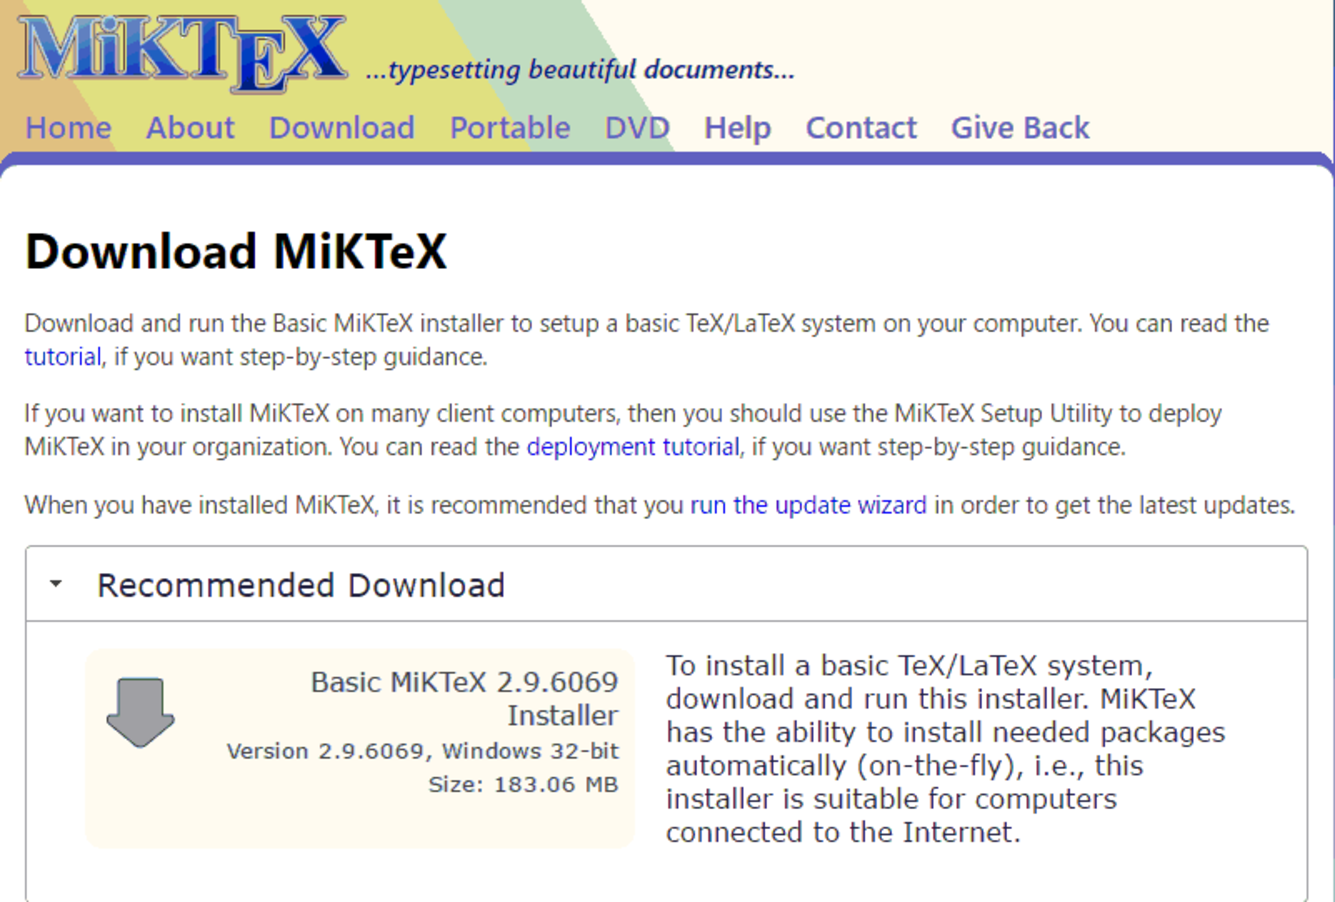
\includegraphics[width=3in]{../images/miktex-download.pdf}
        \caption{MiKTeX download}
        \label{img:MiKTeX download}
    \end{figure}

    \begin{figure}[!hb]
        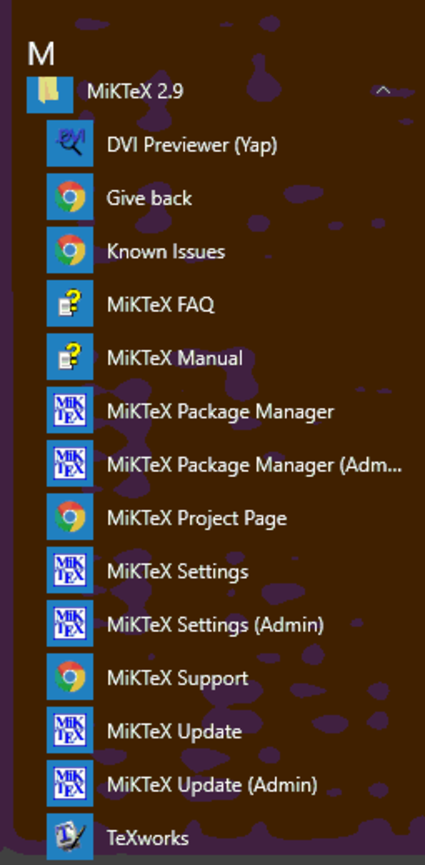
\includegraphics[width=1in]{../images/miktex-winstart.pdf}
        \caption{MiKTeX on Windows start menu}
        \label{img:MiKTeX winstart}
    \end{figure}

    \begin{figure}[!hb]
        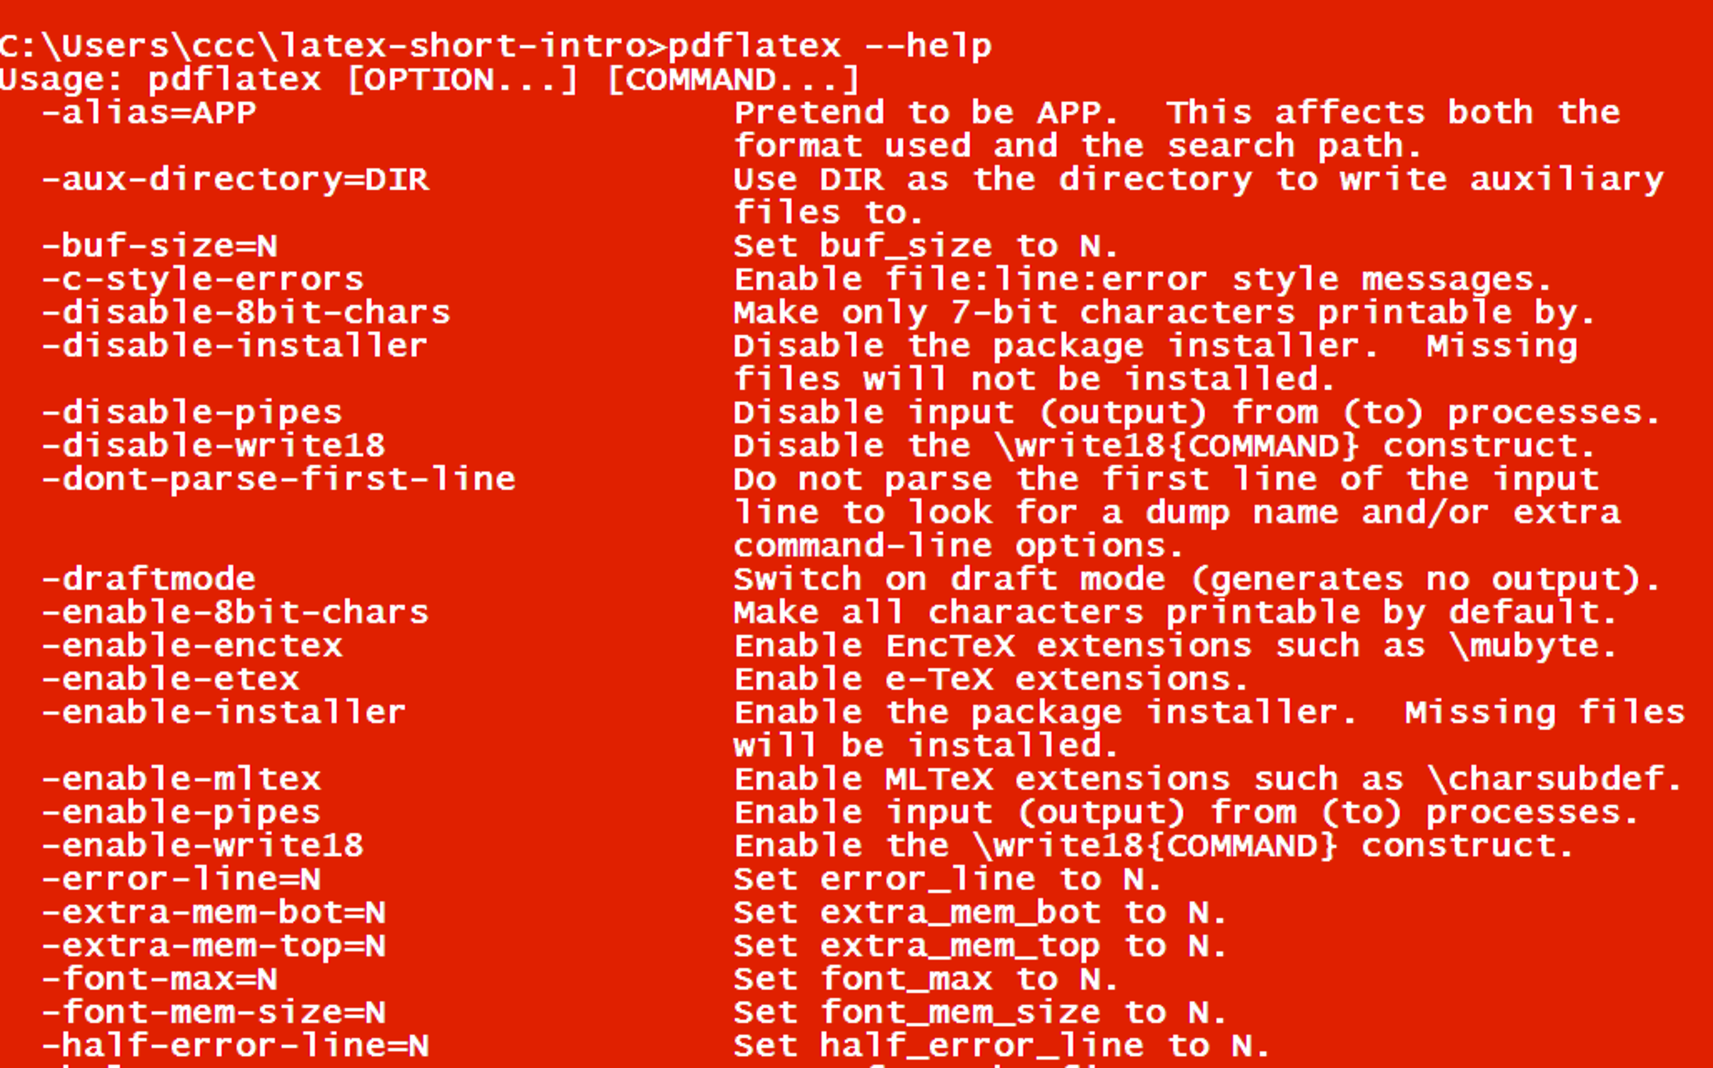
\includegraphics[width=3in]{../images/install-test.pdf}
        \caption{CLI test}
        \label{img:CLI test}
    \end{figure}

    \section{\LaTeXe Editors}
    \label{Editors}

    A \texttt{tex} file is just ordinary plain text, without any special codes or binary commands. You write your \Lx{} document using an ordinary text editor. You can use your favorite text editor with no restrictions, from Windows Notepad (the most minimal text editor I know) on up.\footnote{But be careful of Notepad. Notepad by default saves documents with the \texttt{txt} extension, i.e., as a plain text file. You \textit{must} save your \Lx{} file with a \texttt{tex} extension. Be sure to select the All Files option in the Save As box, and explicitly add \texttt{.tex} to the name of your file}

    Notepad++ is a very popular, full featured, free text editor, and I recommend it for a large number of applications, including \Lx{}. You can find Notepad++ at \url{https://notepad-plus-plus.org/}. Notepad++ is just a text editor, so it doesn't come with any special bells and whistles.\footnote{If you really want to add a compilation feature to Notepad++, search the internet. It's not hard, but I don't cover it here.} Personally, I use \texttt{gvim} as my text editor, as it works for virtually everything, and works on Windows, Mac, Linux, and UNIX. However, \texttt{gvim} requires a substantial investment of time and effort to achieve proficiency, and I don't cover it here.

    Typically, a new user of \Lx{} will choose to use an integrated development which combines a text editor and compiler (see appendix \ref{Development Environments}) or an online resource (see appendix \ref{Online}). Use of a text editor requires separate editing and compilation cycles, which does offer some advantages, which is why some people choose to do it this way.

    \section{Development Environments}
    \label{Development Environments}

    MiKTeX comes with TeXwriter, which combines a text editor with a compiler. It's pretty minimal and crude, but that means that there's less to learn and less to break. Many other \Lx{} programs can be had, both free and commercial. Look at the Wikipedia entry on \Lx{} or \TeX{} editors. TeXmaker is also popular. The advantage to a development environment is that you can do your writing, editing, compilation, and publishing with one application. These also offer nice features, such as syntax coloring, autocomplete, and builtin help systems. The top end development environments also have point and click, drag and drop, features. This results in something close to a blend of a word processor (like Microsoft Word) and \Lx{}. Whether or not this is a good thing is a matter of opinion. You will find that people who use \Lx{} professionaly do not use these kinds of graphical interfaces --- there are very good reasons for this avoidance that you will come to see if you use \Lx{} frequently.

    \section{Online \LaTeXe}
    \label{Online}

    You can also use online \Lx{} editors. There are many equation editors that translate equations into \Lx{} source code. There are also full fledged online \Lx{} systems, which alalow collaboration between colleages. Many (virtually all) are commercial. I have never used any of these so I can't offer an opinion about them. If you do not have an adequate computer (such as a Chromebook, perhaps), online document writing is an option.

    \section{Command Line Execution}
    \label{Command Line}

    Both \TeX{} and \Lx{} consist of executable computer programs that can be invoked and executed on the command line. If you automate your processes (perhaps you have to create lengthy reports several times a day or a week) you will write programs that call these executables to produce your documents. The three commands you will use most often are \texttt{pdflatex}, \texttt{makeindex}, and \texttt{bibtex}. Power users commonly do their work on the command line, and again, there are good reasons for this.

    If the thought of the command line terrifies you, you never have to see it. However, it's always there lurking in the background. And sometimes, use of the command line is the only way to perform some tasks that your GUI program does not implement.




    \theendnotes{}
    \addcontentsline{toc}{section}{Endnotes}

    \bibliographystyle{IEEEtranS}    
    \bibliography{tut}
    \addcontentsline{toc}{section}{References}
    \nocite{*}

    \addcontentsline{toc}{section}{Index}
    \printindex{}

\end{document}

%        \subsection{}
%        \label{}
%        
%        \begin{framed}
%            \begin{itemize}
%                \item{}
%            \end{itemize}
%        \end{framed}
%
%
%        \begin{verbatim}
%\documentclass{article}
%    \title{This is My Title}
%    \author{Charles Carter}
%    \date{\today{}}
%\begin{document} 
%    \maketitle{}
%    \section{Introduction}
%    \label{Introduction}
%    \section{Body}
%    \label{Body}
%    \section{Conclusion}
%    \label{Conclusion}
%\end{document}    
%        \end{verbatim}
%
%        \paragraph{Exercise:}
%
%        \paragraph{Exercise:}


